\section{Maquettage}
\sectitle{Maquettage du site}

\begin{frame}
    \frametitle{Réflexions préliminaires}

    \begin{itemize}
        \item Définition des besoins du site (\textbf{réunions hebdomadaires}).
        \item Analyse des améliorations par rapport à l’ancien site.
        \item Étude de faisabilité en lien avec le \textbf{RGPD}.
    \end{itemize}
\end{frame}

\begin{frame}
    \frametitle{Les fonctionnalités du site}

    \begin{itemize}
        \item \textbf{Présentation de l’association} et de son histoire.
        \item \textbf{Gestion des événements} (inscriptions et suivi).
        \item \textbf{Page d’actualités}.
        \item \textbf{Boutique en ligne} (adhésion et produits).
        \item \textbf{Galerie photo}.
        \item \textbf{Espace administrateur} (gestion des événements, photos, etc.).
        \item \textbf{Système de comptes} (utilisateurs et administrateurs).
        \item \textbf{Jeu ludique} inspiré de \textit{Space Invaders}.
    \end{itemize}
\end{frame}

\begin{frame}
    \frametitle{Choix des technologies}

    \begin{itemize}
        \item Outil de gestion de projet : \textbf{Trello}.
        \item Serveur : choix d’un framework \textbf{PHP}.
        \item Comparaison \textbf{Laravel} vs \textbf{Symfony} :
              \begin{itemize}
                \item Laravel : approche fonctionnelle, plus simple mais moins familière.
                \item Symfony : approche orientée objet, plus adaptée à nos compétences.
              \end{itemize}
        \item Décision finale : \textbf{Symfony} pour sa maintenabilité et son usage répandu en France.
    \end{itemize}
\end{frame}

\begin{frame}
    \frametitle{Maquettage du site}

    \begin{itemize}
        \item Conception en \textbf{deux étapes} :
              \begin{itemize}
                \item \textbf{Esquisse manuscrite} pour organiser les pages.
                \item \textbf{Maquette numérique} réalisée sur \textbf{Figma}.
              \end{itemize}
        \item Validation et ajustements après échanges avec les tuteurs.
        \item Réflexion sur la maintenabilité (\textbf{gestion de contenu sans code}).
    \end{itemize}
\end{frame}

\begin{frame}
    \frametitle{Exemples de maquettes}

    \begin{minipage}{0.48\textwidth}
        \centering
        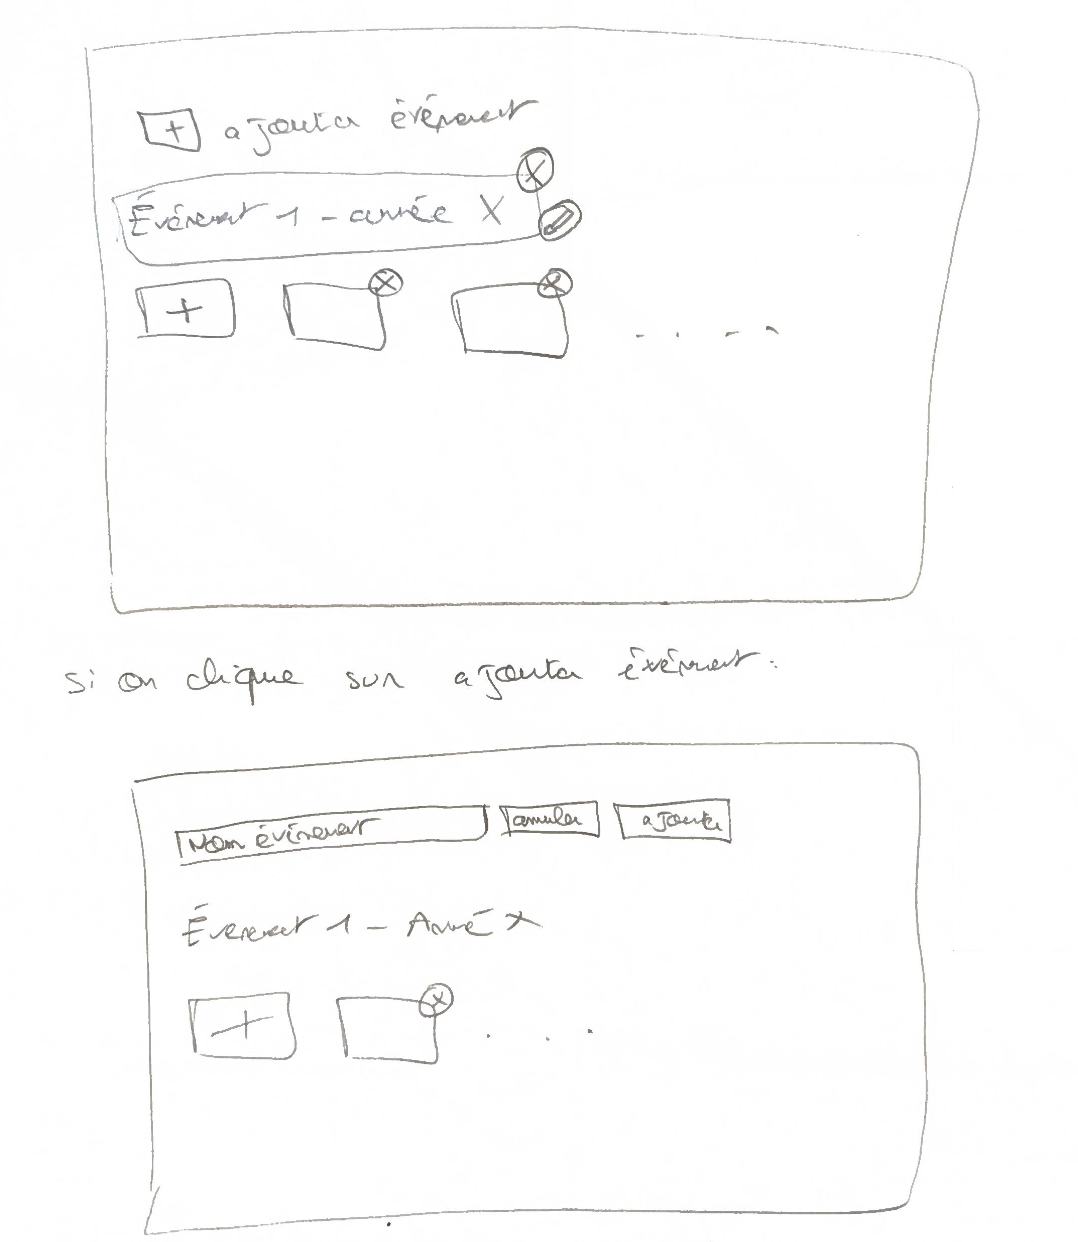
\includegraphics[width=\linewidth]{pictures/maquette.png}
        %\captionof{figure}{Esquisse manuscrite}
    \end{minipage}
    \hfill
    \begin{minipage}{0.48\textwidth}
        \centering
        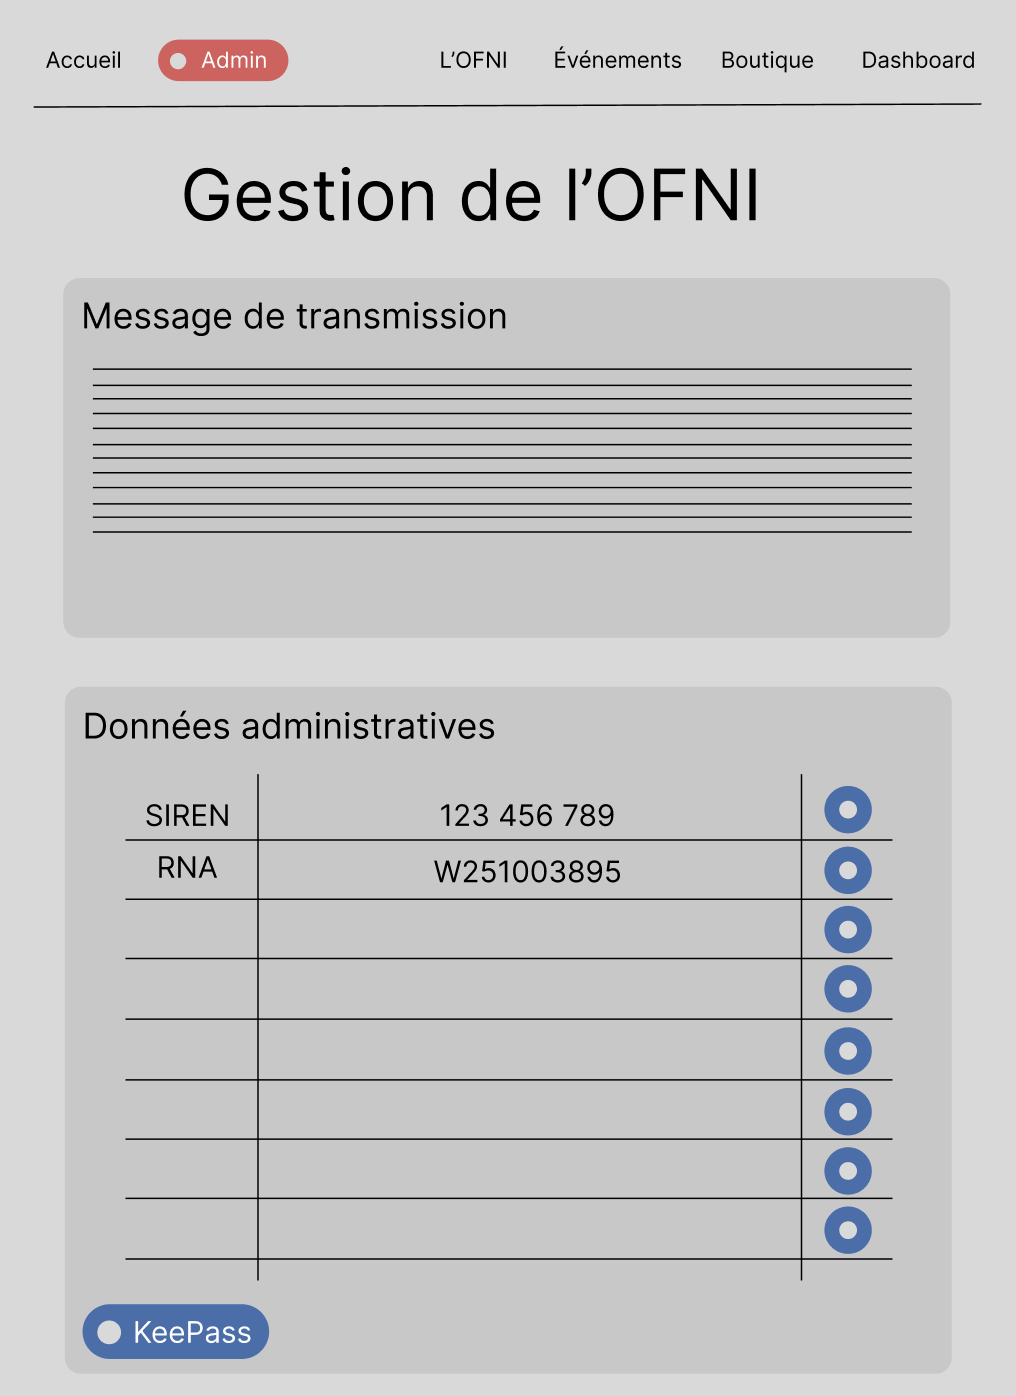
\includegraphics[width=\linewidth]{pictures/figma.png}
        %\captionof{figure}{Maquette numérique}
    \end{minipage}
\end{frame}
